\chapter{Исследовательский раздел}
\label{cha:research}

\section{Тестирование производительности}

\section{Описание используемых шаблонов проектирования}

Для проведения исследования были выбраны следующие шаблоны проектирования:
\begin{itemize}
\item <<абстрактная фабрика>> --- предоставляет интерфейс для создания групп
связанных или зависимых объектов, не указывая их конкретный класс;
\item <<адаптер>> --- конвертирует интерфейс класса в другой интерфейс,
ожидаемый клиентом. Позволяет классам с разными интерфейсами работать вместе;
\item <<вызов переопределенного метода>> --- представляет ситуацию,
когда вызывается метод интерфейса,
для которого имеется реализация в производном классе.
Не является полноценным шаблоном проектирования, а скорее некоторым элементом.
Рассматривается, чтобы убедиться в возможности находить самые простые конструкции;
\item <<декоратор>> --- динамически предоставляет объекту дополнительные
возможности.
Представляет собой гибкую альтернативу наследованию для расширения
функциональности.
\item <<мост>> --- разделяет абстракцию и реализацию так,
чтобы они могли изменяться независимо.
\item <<посетитель>> --- представляет операцию, которая будет выполнена над
объектами группы классов.
Даёт возможность определить новую операцию без изменения кода классов,
над которыми эта операция производится.
\item <<хранитель>> --- не нарушая инкапсуляцияю, определяет и сохраняет
состояние объекта и позволяет восстановить объект в этом состоянии.
\item <<цепочка ответственности>> --- избегает связывания отправителя запроса с
его получателем, давая возможность обработать запрос более чем одному объекту.
Связывает объекты-получатели и передает запрос по цепочке, пока объект не
обработает его.
\end{itemize}

Графы моделей шаблонов представлены в приложении~Е.

\section{Поиск шаблонов проектирования в существующих программах}

\subsection{Проект <<java-design-patterns>>}

Проект находится в открытом доступе, размещен на ресурсе
github.com~\cite{java-design-patterns}.
Интересен тем, что содержит сборник из 48 примеров реализации различных
шаблонов проектирования на языке \textbf{Java},
что очень хорошо подходит для проверки работы программного комплекса.
Здесь можно увидеть некоторые из особенностей реализации шабонов,
поэксперементировать с разными представлениями шаблона.

\subsubsection*{Поиск шаблона <<абстрактная фабрика>>}

Первый реализованный пример шаблона в проекте.
Реализация совпадает с разными описаниями.
Шаблон находится, результат представлен на рисунке~\ref{fig:java-design-patterns-abstract-factory}.

\begin{figure}[!ht]
\centering
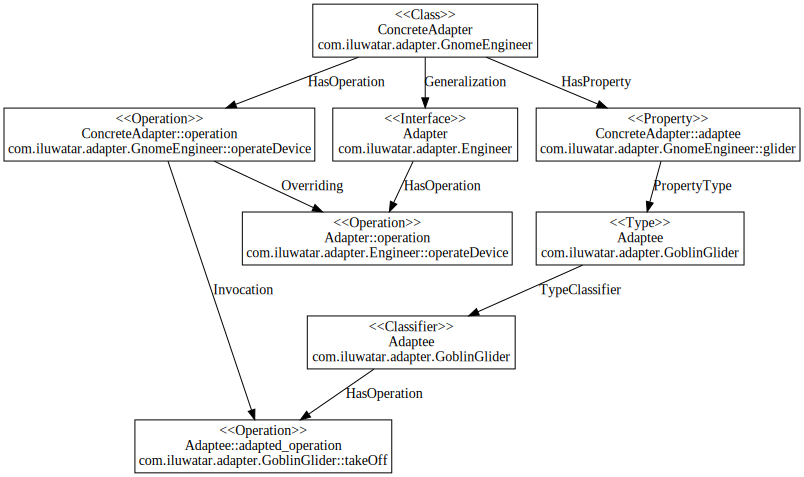
\includegraphics[width=\textwidth]{inc/java-design-patterns-adapter.pdf}
\caption{Результат поиска шаблона проектирования <<абстрактная фабрика>> в примере его реализации}
\label{fig:java-design-patterns-abstract-factory}
\end{figure}

\subsubsection*{Поиск шаблона <<адаптер>>}

Для шаблона есть пример, и шаблон в нем находится.
Результат представлен на рисунке~\ref{fig:java-design-patterns-adapter}

\begin{figure}[!ht]
\centering
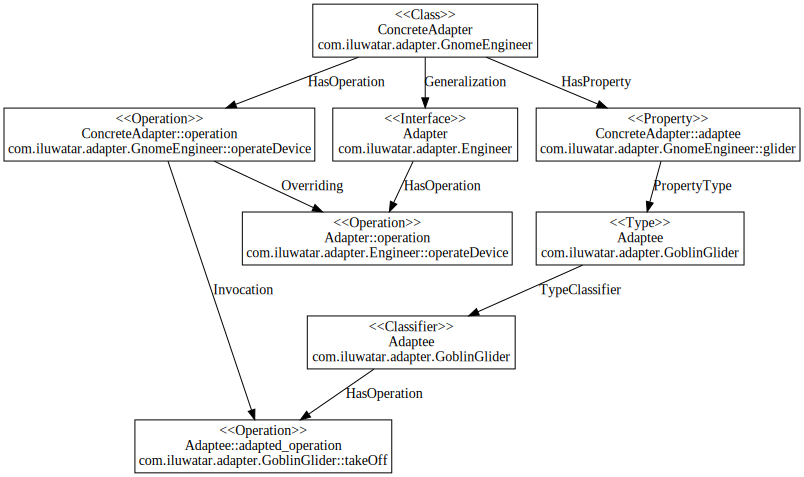
\includegraphics[width=\textwidth]{inc/java-design-patterns-adapter.pdf}
\caption{Результат поиска шаблона проектирования <<адаптер>> в примере его реализации}
\label{fig:java-design-patterns-adapter}
\end{figure}

\subsubsection*{Поиск шаблона <<мост>>}

В примере реализации не найден, но найден в других примерах.
Проблема заключается в том, что используется дополнительное обобщение,
чтобы не было дублирования кода.
Класс \textbf{Abstraction} разделен на две части: базовый абстрактный класс
\textbf{MagicWeapon},
который совязан ассоциацией с \textbf{MagicWeaponImp},
являющимся интерфейсом \textbf{Implementor};
и конкретными реализацими: \textbf{BlindingMagicWeapon},
\textbf{FlyingMagicWeapon}, \textbf{SoulEatingMagicWeapon}.
Здесь требуется механизм, который позволит описать класс так,
все ассоциации базового класса также являются и ассоциациями производного.
Нужна сущность, которая может объединять иерархии наследования классов в
некоторый надкласс.
UML-диаграммы классов не предоставляют такого механизма.
В данной работе эта проблема осталась не решенной.

Шаблон был найден в следующих примерах:
\begin{itemize}
\item adapter;
\item decorator;
\item intercepting-filter;
\item mediator;
\item model-view-presenter;
\item null-object;
\item poison-pill;
\item property;
\item service-layer;
\item state;
\item strategy.
\end{itemize}

\subsubsection*{Поиск шаблона <<посетитель>>}

Шаблон реализован в специальном примере и находится.
Результат представлен на рисунке~\ref{fig:java-design-patterns-visitor}

\begin{figure}[!ht]
\centering
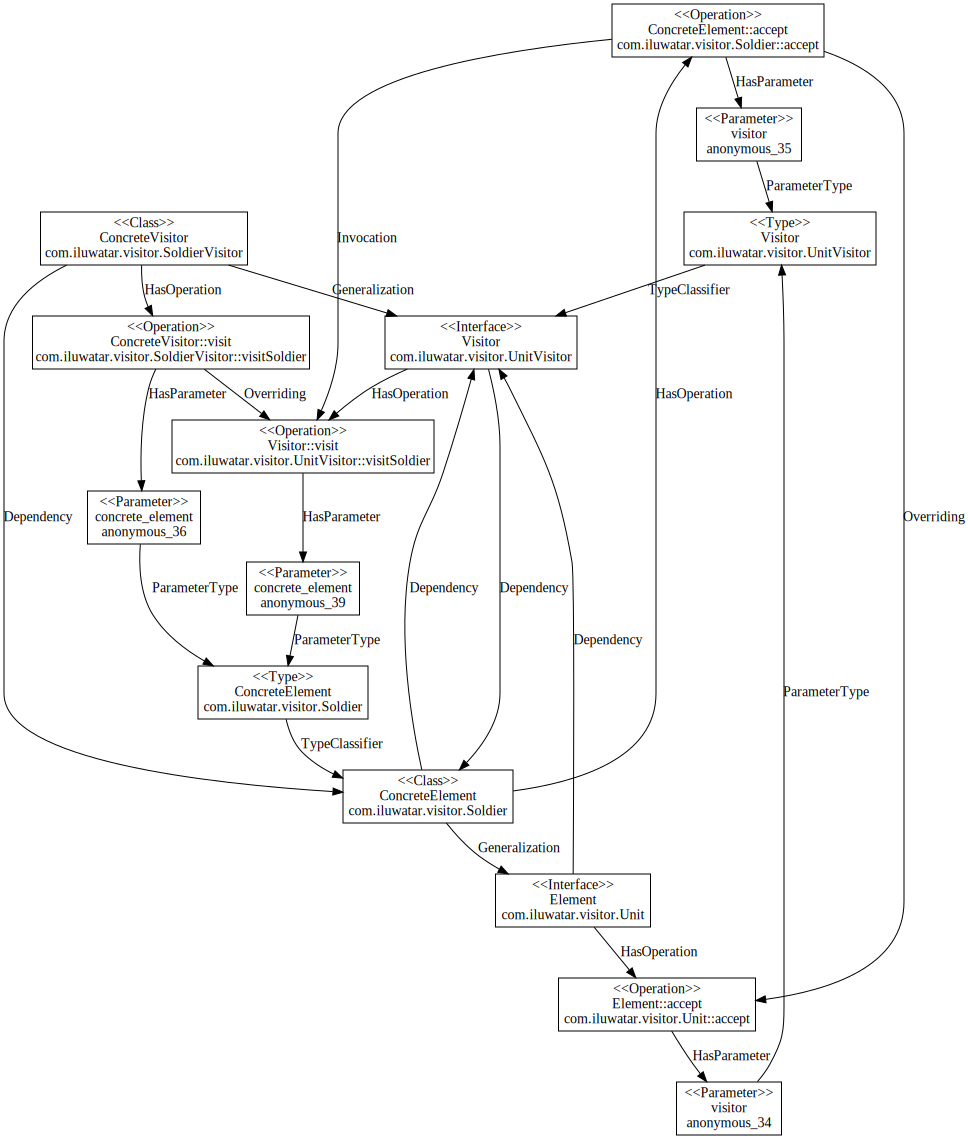
\includegraphics[width=\textwidth]{inc/java-design-patterns-visitor.pdf}
\caption{Результат поиска шаблона проектирования <<посетитель>> в примере его реализации}
\label{fig:java-design-patterns-visitor}
\end{figure}

\subsection{Библиотека <<Apache BCEL>>}

Исследовалась в качестве примера реального проекта.
Модель проекта в \textbf{YAML}-формате занимает 4,1 МБ.
Граф модели состоит из 7700 вершин и 52000 дуг.
Здесь были найдены шаблоны <<адаптер>> (см. рисунок~\ref{fig:apache-bcel-adapter}),
<<мост>> (см. рисунок~\ref{fig:apache-bcel-bridge}).
Другие шаблоны не найдены.

\begin{figure}[!ht]
\centering
\includegraphics[width=\textwidth]{inc/apache-bcel-adapter.pdf}
\caption{Результат поиска шаблона проектирования <<адаптер>> в <<Apache BCEL>>}
\label{fig:apache-bcel-adapter}
\end{figure}

\begin{figure}[!ht]
\centering
\includegraphics[width=\textwidth]{inc/apache-bcel-bridge.pdf}
\caption{Результат поиска шаблона проектирования <<мост>> в <<Apache BCEL>>}
\label{fig:apache-bcel-bridge}
\end{figure}

\subsection{Поиск шаблонов проектирования в других проектах}

Исследовались другие проекты, написанные на языках \textbf{Java} и один на \textbf{Scala}.
Сводные результаты по всем проектам приведены в таблице~\ref{table:other-projects}.

\begin{table}[ht!]
    \centering
    \begin{tabulary}{\textwidth}{|C|C|C|}
        \hline
        Название проекта & Язык~\quad & Найденные шаблоны проектирования \\
        \hline
        Netflix EVCacahe & Java & <<вызов переопределенного метода>>, <<мост>> \\
        \hline
        airbnb aerosolve & Java & <<вызов переопределенного метода>>, <<мост>> \\
        \hline
        java-design-patterns & Java & <<абстрактная фабрика>>, <<адаптер>>, <<мост>>, <<посетитель>>, <<вызов переопределенного метода>> \\
        \hline
        Apache BCEL & Java & <<адаптер>>, <<вызов переопределенного метода>>, <<мост>> \\
        \hline
        Apache Zookeeper & Java & <<вызов переопределенного метода>>, <<мост>> \\
        \hline
        scodec & Scala & <<вызов переопределенного метода>> \\
        \hline
    \end{tabulary}
    \caption{Результаты поиска шаблонов проектирования в различных проектах}
    \label{table:other-projects}
\end{table}

\subsection{Выводы по результатам исследования}

Метод позволяет находить шаблоны проектирования.
<<Вызов переопределенного метода>> встречается во всех проектах.
Это одна из самых распространненых конструкций.
Имеено для этого существует разделение между интерфейсом и реализацией.
Не удивительно, что такую базовую возможность ООП используют везде.
Наиболее часто встречаются шаблоны проектирования <<адаптер>> и <<мост>>.
Можно утверждать, что модели достаточно хорошо отражают эти шаблоны, и что
они действительно используются.
Для других шаблонов можно предположить, что они предназначены для специфических задач,
которые не решались в рассматриваемых проектах.
